% !TEX root = doc.tex
% Copyright (c) 2017 The ALF project.
% This is a part of the ALF project documentation.
% The ALF project documentation by the ALF contributors is licensed
% under a Creative Commons Attribution-ShareAlike 4.0 International License.
% For the licensing details of the documentation see license.CCBYSA.
%



%-----------------------------------------------------------------------------------
\subsection{The Trotter error and  checkerboard  decomposition }\label{sec:trotter}
%-----------------------------------------------------------------------------------
%

\subsubsection{Asymmetric  Trotter decomposition}
In practice, many applications are carried out at finite  imaginary time steps,  and it is important to  understand the consequences of the Trotter error.
How does it scale with system size and  what  symmetries  does it break?
In particular, when investigating a critical point, one should determine whether the potential symmetry breaking  associated  with the Trotter decomposition generates relevant operators.

To best describe the workings of the ALF  code,  we divide the Hamiltonian into  hopping terms  $\hat{\mathcal{H}}_{T}$  and interaction terms  
$\hat{\mathcal{H}}_{V} +  \hat{\mathcal{H}}_{I}   +   \hat{\mathcal{H}}_{0,I} $.       Let 
\begin{align}
\label{Checkerboard.Eq}
	\hat{\mathcal{H}}_{T}     = \sum_{i=1}^{N_T} \sum_{k \in \mathcal{S}^{T}_i} \hat{T}^{(k)}  \equiv \sum_{i=1}^{N_T} \hat{T}_{i}.
\end{align}
Here the decomposition follows the rule  that if $k$ and $k'$  belong to the same set $\mathcal{S}^{T}_i $ then   $ \left[ \hat{T}^{(k)} , \hat{T}^{(k')} \right] = 0 $.  An important case to consider is that of the checkerboard decomposition.
For the square lattice we can decouple the nearest neighbor hopping  into $N_T=4$ groups,  each consisting of two site hopping processes.
This type of checkerboard decomposition is activated for a set  of predefined lattices by setting the flag \index{\texttt{Checkerboard}} \texttt{Checkerboard} to \texttt{.true.}.
We will carry out the same separation for the interaction: 
\begin{equation}
	\hat{\mathcal{H}}_{V}  +  \hat{\mathcal{H}}_{I}   +   \hat{\mathcal{H}}_{0,I}   = \sum_{i=1}^{N_I}  \hat{O}_{i},
\end{equation}
where each $\hat{O}_{i}$  contains a set of commuting terms.  For instance, for the Hubbard model,   the  above reduces to 
$U \sum_{\vec{i}}  \hat{n}_{\vec{i},\uparrow } \hat{n}_{\vec{i},\downarrow }  $    such that $N_I = 1$ and   $ \hat{O}_{1} = U \sum_{\vec{i}}  \hat{n}_{\vec{i},\uparrow } \hat{n}_{\vec{i},\downarrow }   $. 

The default Trotter decomposition in the ALF code is  based on the equation: 
\begin{equation}
	e^{ -\Delta \tau \left( \hat{A} + \hat{B} \right)  }  =  e^{ -\Delta \tau \hat{A}}  e^{ -\Delta \tau  \hat{B}  }   +  \frac{\Delta  \tau^2}{2} \left[ \hat{B}, \hat{A} \right] + \mathcal{O} \left (\Delta \tau ^3 \right).
\end{equation}
Using iteratively the above  the single time step is given by: 
\begin{multline}
    e^{-\Delta \tau \mathcal{H}}   =   \prod_{i=1}^{N_O} e^{-\Delta \tau \hat{O}_i} \prod_{j=1}^{N_T} e^{-\Delta \tau \hat{T}_j}   \\
    + \underbrace{ \frac{\Delta \tau^2}{2}  
   \left(    \sum_{i=1}^{N_O}  \sum_{j=1}^{N_T} \left[ \hat{T}_j, \hat{O}_i \right]  +   \sum_{j'}^{N_T -1}  \left[ \hat{T}_{j'},   \hat{T}_{j'}^{>}\right] 
   +   \sum_{i'=1}^{N_O-1}  \left[ \hat{O}_{i'}, \hat{O}^{>}_{i'} \right]  \right)  }_{\equiv \Delta \tau \hat{\lambda}_1} 
   + \mathcal{O} \left( \Delta \tau^3 \right).
\end{multline}
In the above, we have introduced the shorthand notation 
\begin{equation}
\hat{T}_{n}^{>} = \sum_{j=n+1}^{N_T}  \hat{T}_{j} \; \text{ and } \; \hat{O}_{n}^{>} = \sum_{j=n+1}^{N_O}  \hat{O}_{j}.
\end{equation} 
The full propagation then reads
\begin{equation}
\begin{split}
  \hat{U}_{\text{Approx}} &=  \left(\prod_{i=1}^{N_O} e^{-\Delta \tau \hat{O}_i} \prod_{j=1}^{N_T} e^{-\Delta \tau \hat{T}_j}  \right)^{\!\!L_\text{Trotter}} \!  = e^{-\beta \left(  \hat{H} + \hat{\lambda}_1 \right)} 
  + \mathcal{O} \left( \Delta \tau^2 \right)  \\
  &=  e^{-\beta  \hat{H}  }  - 
	 \int_0^{\beta}  d \tau  e^{-(\beta-\tau )\hat{H}} \hat{\lambda}_1  e^{-\tau \hat{H}}   +  \mathcal{O} (\Delta \tau^2 ).
\end{split}
\end{equation} 
The last step follows from time-dependent perturbation theory. 
The following comments are in order:
\begin{itemize}
\item    The error is anti-Hermitian  since $\hat{\lambda}_1^{\dagger} = - \hat{\lambda}_1 $. As a consequence, if all the operators as well as the quantity being measured are simultaneously real representable,  then   the prefactor of the linear in $\Delta  \tau$ error vanishes since it ultimately corresponds to computing the trace of an  anti-symmetric matrix. This \textit{lucky}   cancellation was put forward in  Ref.~\cite{Fye86}.   Hence, under this assumption -- which is certainly valid for the Hubbard model considered in Fig.~\ref{Trotter.fig} -- the systematic error is of order $\Delta \tau^2$.
\item  The biggest drawback  of the above decomposition is that  the imaginary-time propagation is not Hermitian.   This can lead to acausal  features in imaginary-time correlation functions \cite{Beyl_thesis}. To be more precise, the eigenvalues of  
$  H_{\text{Approx}} = - \frac{1}{\beta} \log  U_{\text{Approx}}$ need not be real and thus imaginary-time displaced correlation functions may oscillate as a function of imaginary time.   
This is shown in  Fig.~\ref{Trotter.fig}(a)  that plots the  absolute value of local time-displaced Green function for  the Honeycomb lattice at $U/t=2$.  Sign changes of this quantity   involve zeros  that, on the considered log-scale,  correspond to negative divergences.
As detailed in \cite{goth2020} using the non-symmetric Trotter decomposition 
leads to an additional second order error in the measurement of observables $O$
that is $\propto [T,[T,O]]$.
As we see next, these issues can be solved by considering a symmetric  Trotter decomposition.
\end{itemize}


\subsubsection{Symmetric Trotter decomposition} 

To address the issue described above, the ALF package provides the possibility of using a symmetric Trotter decomposition,
\begin{equation}
	e^{ -\Delta \tau \left( \hat{A} + \hat{B} \right)  }  =  e^{ -\Delta \tau \hat{A/2}}  e^{ -\Delta \tau  \hat{B}  }   e^{ -\Delta \tau \hat{A/2}}  +  \frac{\Delta  \tau^3}{12} \left[ 2\hat{A} + \hat{B}, \left[\hat{B}, \hat{A} \right]\right] + \mathcal{O} \left (\Delta \tau ^5 \right),
\end{equation}
by setting the \texttt{Symm} \index{\texttt{Symm}} flag to \texttt{.true.}.
Before we apply the expression above to a time step, let us write
\begin{equation}
	e^{-\Delta \tau \mathcal{H}}    =       e^{-\frac{\Delta \tau}{2} \sum_{j=1}^{N_T} \hat{T}_j } e^{-\Delta \tau \sum_{i=1}^{N_I} \hat{O}_i } e^{-\frac{\Delta \tau}{2} \sum_{j=1}^{N_T} \hat{T}_j }   
	 +  \underbrace{\frac{\Delta \tau ^3}{12}   \left[ 2\hat{T}^{>}_0 + \hat{O}^{>}_0, \left[\hat{O}^{>}_{0}, \hat{T}^{>}_0 \right]\right] }_{\equiv \Delta \tau \hat{\lambda}_{TO}}   + \mathcal{O}\left(  \Delta \tau^5 \right).
\end{equation}
Then,
\begin{multline}
 e^{-\Delta \tau \sum_{i}^{N_I} \hat{O}_i }  =  \left(\prod_{i=1}^{N_O-1} e^{-\frac{\Delta \tau}{2} \hat{O}_i } \right)    e^{-\Delta \tau \hat{O}_{N_O} }    
   \left(  \prod_{i=N_O-1}^{1} e^{-\frac{\Delta \tau}{2} \hat{O}_i } \right)   \\
  + \underbrace{\frac{\Delta \tau ^3}{12}  \sum_{i=1}^{N_0-1} \left[ 2\hat{O}_i + \hat{O}^{>}_i, \left[\hat{O}^{>}_{i}, \hat{O}_i \right]\right] }_{\equiv \Delta \tau \hat{\lambda}_{O}}    + \mathcal{O}\left(  \Delta  \tau^5 \right), 
\end{multline}
\begin{multline}
 e^{- \frac{\Delta \tau}{2} \sum_{j}^{N_T} \hat{T}_j }  = \left(\prod_{j=1}^{N_T-1} e^{-\frac{\Delta \tau}{4} \hat{T}_j } \right)    e^{-\frac{\Delta \tau}{2} \hat{T}_{N_T} }    
   \left(  \prod_{j=N_T-1}^{1} e^{-\frac{\Delta \tau}{4} \hat{T}_j } \right)  \\
  + \underbrace{\frac{\Delta \tau ^3}{96}  \sum_{j=1}^{N_T-1} \left[ 2\hat{T}_j + \hat{T}^{>}_j, \left[\hat{T}^{>}_{j}, \hat{T}_j \right]\right] }_{\equiv \Delta \tau \hat{\lambda}_{T}}    + \mathcal{O}\left(  \Delta  \tau^5 \right) 
\end{multline}
and we can derive  a  closed equation  for  the free energy density:
\begin{align}
f_{\text{Approx} }  &=  
\begin{aligned}[t]
   -\frac{1}{\beta V } \log \Tr &\left[ \left(\prod_{j=1}^{N_T-1} e^{-\frac{\Delta \tau}{4} \hat{T}_j } \right)    e^{-\frac{\Delta \tau}{2} \hat{T}_{N_T} } \;   
   \left(  \prod_{j=N_T-1}^{1} e^{-\frac{\Delta \tau}{4} \hat{T}_j } \right)  \times   \right. \nonumber \\   
   &\;\;\left(\prod_{i=1\phantom{N_O}}^{N_O-1} e^{-\frac{\Delta \tau}{2} \hat{O}_i } \right)    e^{-\Delta \tau \hat{O}_{N_O} }    
     \left( \prod_{i=N_O-1}^{1} e^{-\frac{\Delta \tau}{2} \hat{O}_i } \right)  \times  \nonumber  \\
   &\;\;\left.   \left(\prod_{j=1}^{N_T-1} e^{-\frac{\Delta \tau}{4} \hat{T}_j } \right)    e^{-\frac{\Delta \tau}{2} \hat{T}_{N_T} }  \;  
   \left(  \prod_{j=N_T-1}^{1} e^{-\frac{\Delta \tau}{4} \hat{T}_j } \right)   
   \right]^{L_{\text{Trotter}}}  \nonumber 
\end{aligned}\\
   &= f    - \frac{1}{V}   \langle \hat{\lambda}_{TO} + \hat{\lambda}_{O} + 2 \hat{\lambda}_{T} \rangle  + \mathcal{O}( \Delta \tau ^4).
\end{align}

The following comments are in order:
\begin{itemize}
\item   The approximate imaginary-time propagation from which the $f_{\text{Approx} } $ is derived is Hermitian.  Hence no spurious effects in imaginary-time correlation functions are to be expected.  This is clearly shown in Fig.~\ref{Trotter.fig}(a).
\item  In Fig.~\ref{Trotter.fig}(b) we  have used the ALF-library with   \texttt{Symm=.true.} \index{\texttt{Symm}} with and without checkerboard decomposition.  We still expect the systematic error to be of order $\Delta \tau ^2 $.  However its prefactor is much smaller than that of the aforementioned  anti-symmetric decomposition.
\item   We have taken the burden to evaluate explicitly the prefactor of the $\Delta \tau ^2$ error on the free energy density.  One can  see that for Hamiltonians  that are sums of local  operators, the quantity $ \langle \hat{\lambda}_{TO} + \hat{\lambda}_{O} + 2 \hat{\lambda}_{T} \rangle  $ scales as the volume $V$  of the system, such that the systematic error on the free energy density (and on correlation functions that can be computed  by adding source terms)  will be  volume  independent. For model  Hamiltonians that are not sums of local terms, care must be taken.  A conservative upper bound on the  error is $ \langle \hat{\lambda}_{TO} + \hat{\lambda}_{O} + 2 \hat{\lambda}_{T} \rangle    \propto \Delta \tau^2 V^3 $, which means that, in order to maintain a constant systematic error for the free energy density, we have to keep $ \Delta \tau V $ constant. Such a situation has been observed in Ref.~\cite{WangZ20}.
\end{itemize}


\begin{figure}
\center
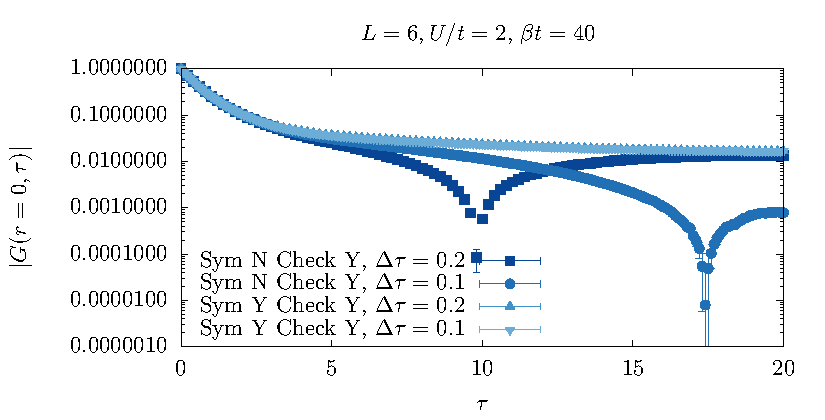
\includegraphics[width=0.49\textwidth]{Figures/Dtau_1/Dtau_1.pdf}
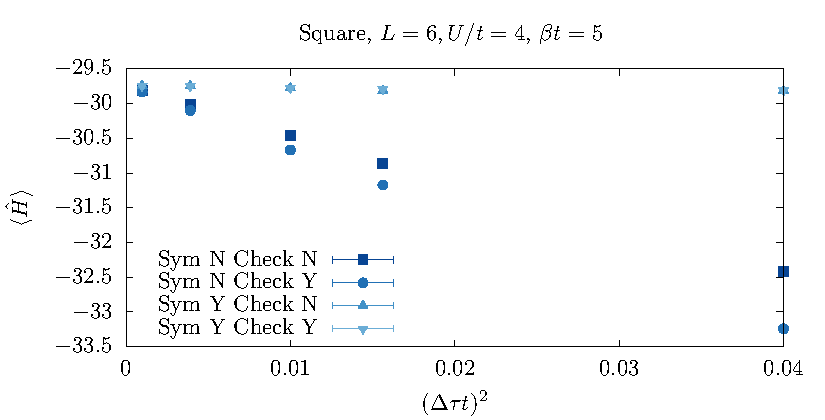
\includegraphics[width=0.49\textwidth]{Figures/Dtau/Dtau.pdf}

\caption{Analysis of  Trotter systematic error.
        Left:    We consider a $6 \times 6$ Hubbard model on the Honeycomb lattice, $U/t=2$, half-band filling,  inverse temperature $\beta t =40$,  and we have used an HS transformation that couples to  the density.    The figure plots the  local-time displaced Green function.
        Right: Here we consider the $6\times 6$ Hubbard model at $U/t=4$, half-band filling,  inverse temperature $\beta t =5$, and we have used the HS transformation that couples to the $z$-component of spin.  We provide data for the four combinations of  the logical variables \texttt{Symm}  and \texttt{Checkerboard}, where  \texttt{Symm=.true.}  (\texttt{.false.})  indicates a symmetric  (asymmetric) Trotter decomposition has been used, and  \texttt{Checkerboard=.true.}  (\texttt{.false.})   that the checkerboard decomposition for the hopping matrix has (not) been used.
        The large deviations between different choices of \texttt{Symm} are here $\sim [T, [T,H]]$ as detailed in \cite{goth2020}.
  }
        \label{Trotter.fig}
\end{figure}

Alternative symmetric second order methods as well as the issues with decompositions of higher order 
have been detailed in \cite{goth2020}.

\subsubsection{The \texttt{Symm} flag} 

If the  \texttt{Symm}   \index{\texttt{Symm}} flag is set to true,  then the program will automatically --  for the set of predefined lattices  and models -- use the symmetric   $\Delta \tau$ time step  of the interaction and 
hopping terms.

To save CPU time  when the \texttt{Symm}  flag is on  we  carry out the following   approximation:
\begin{multline}
	\left[  
	  \left(\prod_{j=1}^{N_T-1} e^{-\frac{\Delta \tau}{4} \hat{T}_j } \right)    e^{-\frac{\Delta \tau}{2} \hat{T}_{N_T} }    
   \left(  \prod_{j=N_T-1}^{1} e^{-\frac{\Delta \tau}{4} \hat{T}_j } \right)      \right]^2   \simeq \\
	   \left(\prod_{j=1}^{N_T-1} e^{-\frac{\Delta \tau}{2} \hat{T}_j } \right)    e^{-\Delta \tau\hat{T}_{N_T} }    
   \left(  \prod_{j=N_T-1}^{1} e^{-\frac{\Delta \tau}{2} \hat{T}_j } \right).   
\end{multline}
The above  is consistent with the overall precision of the Trotter decomposition and more importantly  conserves the Hermiticity of the propagation. 

%-----------------------------------------------------------------------------------
\subsection{Stabilization - a peculiarity of the BSS algorithm}\label{sec:stable}
%-----------------------------------------------------------------------------------
%
From the partition function in Eq.~\eqref{eqn:partition_2} it can be seen that, for the calculation of the Monte Carlo weight and of the observables, a long product of matrix exponentials has to be formed.
In addition to that, we need to be able to extract the single-particle Green function  for a given flavor index at, say, time slice $\tau = 0$.  As  mentioned above (cf. Eq.~\eqref{eqn:Green_eq}), this quantity is given by: 
\begin{equation}
\bm{G}= \left( \mathds{1} + \prod_{ \tau= 1}^{L_{\text{Trotter}}} \bm{B}_\tau \right)^{-1},
\end{equation}
which can be recast as the more familiar linear algebra problem of finding a solution for the linear system
\begin{equation}
\left(\mathds{1} + \prod_{\tau=1}^{L_{\text{Trotter}}} \bm{B}_\tau\right) x = b.
\end{equation}
The matrices $\bm{B}_\tau \in \mathbb{C}^{n\times n}$ depend on the lattice size as well as other physical parameters that can be chosen such that a matrix norm of $\bm{B}_\tau$ can be unbound in magnitude.
From standard perturbation theory for linear systems, the computed solution $\tilde{x}$ would 
contain a relative error
\begin{equation}
\frac{|\tilde{x} - x|}{|x|} = \mathcal{O}\left(\epsilon \kappa_p\left(\mathds{1} + \prod_{\tau=1}^{L_{\text{Trotter}}} \bm{B}_\tau\right)\right),
\end{equation}
where $\epsilon$ denotes the machine precision, which is $2^{-53}$ for IEEE double-precision numbers, and $\kappa_p(\bm{M})$ is the condition number of the matrix $\bm{M}$ with respect to the matrix $p$-norm. Due to $\prod_ \tau \bm{B}_\tau$ containing exponentially large and small scales, as can be seen in Eq.~\eqref{eqn:partition_2}, a straightforward inversion is completely ill-suited, in that its condition number would grow exponentially with increasing inverse temperature, rendering the computed solution $\tilde{x}$ meaningless.

In order to circumvent this, more sophisticated methods have to be employed.
In the realm of the BSS algorithm there has been a long history \cite{Loh1989, Sorella89, Assaad02,Loh2005, Bai2011, Bauer2020} of using various matrix factorization techniques.
The predominant techniques are either based on the singular value decomposition(SVD) or 
on techniques using a QR decomposition.
The default stabilization strategy in the auxiliary-field QMC implementation of the ALF package, is then to form a product of QR-decompositions, which was proven to be weakly backwards stable in \cite{Bai2011}. While algorithms using the SVD can provide higher stability 
at a higher cost we note that great care has to be taken in the choice of the right
algorithm for the SVD that achieve the necessary high relative accuracy \cite{Demmel1992, Dongarra2018}.
As a first step we assume that, for a given integer \texttt{NWrap}, the multiplication of \texttt{NWrap} $\bm{B}$ matrices has an acceptable condition number and, for simplicity, that $L_{\text{Trotter}}$ is divisible by \texttt{NWrap}. We can then write:
%\begin{equation}
%\bm{G} = \left( \mathds{1} + \prod\limits_{ i = 0}^{\frac{L_{\text{Trotter}}} {\texttt{NWrap} -1}}       \underbrace{\prod_{\tau=1}^{\texttt{NWrap}} \bm{B}_{i  \cdot  \texttt{NWrap}+ \tau} }_{ \equiv \mathcal{\bm{B}}_i}\right)^{-1}.
%\end{equation}
\begin{equation}
\bm{G} = \Vast( \mathds{1} + \prod\limits_{ i = 1}^{\frac{L_{\text{Trotter}}} {\texttt{NWrap}}}       \underbrace{\prod_{\tau=1}^{\texttt{NWrap}} \bm{B}_{(i-1)  \cdot  \texttt{NWrap}+ \tau} }_{ \equiv \mathcal{\bm{B}}_i} \Vast)^{-1}.
\end{equation}

The key idea is to efficiently separate the scales of a matrix from the orthogonal part of a matrix.
This can be achieved with the QR decomposition of a matrix $\bm{A}$ in the form $\bm{A}_i = \bm{Q}_i \bm{R}_i$. The matrix $\bm{Q}_i$ is unitary and hence in the usual $2$-norm it satisfies $\kappa_2(\bm{Q}_i) = 1$.
To get a handle on the condition number of $\bm{R}_i$ we consider the
diagonal matrix
\begin{equation}
(\bm{D}_i)_{n,n} = |(\bm{R}_i)_{n,n}|
\label{eq:diagnorm}
\end{equation}
and set $\tilde{\bm{R}}_i = \bm{D}_i^{-1} \bm{R}_i$, which gives the decomposition
\begin{equation}
\bm{A}_i = \bm{Q}_i \bm{D}_i \tilde{\bm{R}}_i.
\end{equation}
The matrix $\bm{D}_i$ now contains the row norms of the original $\bm{R}_i$ matrix and hence attempts to separate off the total scales of the problem from $\bm{R}_i$.
This is similar in spirit to the so-called matrix equilibration which tries to improve the condition number of a matrix through suitably chosen column and row scalings.
Due to a theorem by van der Sluis \cite{vanderSluis1969} we know that the choice in Eq.~\eqref{eq:diagnorm} is almost optimal among all diagonal matrices $\bm{D}$ from the space of diagonal matrices $\mathcal{D}$, in the sense that
\begin{equation*}
\kappa_p((\bm{D}_i)^{-1} \bm{R}_i ) \leq n^{1/p} \min_{\bm{D} \in \mathcal{D}} \kappa_p(\bm{D}^{-1} \bm{R}_i).
\end{equation*}
Now, given an initial decomposition $\bm{A}_{j-1} = \prod_i \mathcal{\bm{B}}_i = \bm{Q}_{j-1} \bm{D}_{j-1} \bm{T}_{j-1}$, an update
$\mathcal{\bm{B}}_j \bm{A}_{j-1}$ is formed in the following three steps:
\begin{enumerate}
\item Form $ \bm{M}_j = (\mathcal{\bm{B}}_j \bm{Q}_{j-1}) \bm{D}_{j-1}$. Note the parentheses.
\item Do a QR decomposition of $\bm{M}_j = \bm{Q}_j \bm{D}_j \bm{R}_j$. This gives the final $\bm{Q}_j$ and $\bm{D}_j$.
\item Form the updated $\bm{T}$ matrices $\bm{T}_j = \bm{R}_j \bm{T}_{j-1}$.
\end{enumerate}
This is a stable but expensive method for calculating the matrix product. Here is where \path{NWrap} comes into play: it specifies 
the number of plain multiplications performed between the QR decompositions just described, so that \path{NWrap}~=~1 corresponds to always performing QR decompositions whereas larger values define longer intervals where no QR decomposition will be performed.
%\path{Nwrap} determines the imaginary time interval after which the stabilization is being done.
Whenever we perform a stabilization, we compare the old result (fast updates) with the new one (recalculated from the QR stabilized matrices). The difference is documented as the stability, both for the Green function and for the sign (of the determinant)
The effectiveness of the stabilization \emph{has} to be judged for every simulation from the output file \path{info} (Sec.~\ref{sec:output_obs}). For most simulations there are two values to look out for:
\begin{itemize}
\item \texttt{Precision Green} \index{\texttt{Precision Green} }
\item \texttt{Precision Phase} \index{\texttt{Precision Phase}}
\end{itemize}
The Green function, as well as the average phase, are usually numbers with a magnitude of $\mathcal{O} (1)$. 
For that reason we recommend that \path{NWrap} \index{\path{NWrap}} is chosen such that the mean precision is of the order of $10^{-8}$ or better (for further recommendations see Sec.~\ref{sec:optimize}).
We include typical values of \texttt{Precision Phase} and of the mean and the maximal values of \texttt{Precision Green} in the example simulations discussed in Sec.~\ref{sec:prec_spin}.
